\chapter{Beyond the Standard Model physics program }
\label{ch:bsm}

%%%%%%%%%%%%%%%%%%%%%%%%%%%%%%%%%%%%%%%%%%%%%%%%%%%%%%%%%%%%%%
\section{Beam-induced physics capitalizing on DUNE far detector capabilities}\label{sec:bsm-beam}

\begin{itemize}
\item General Motivation
\item Summary of Difference in Assumptions from Standard Oscillations if applicable (e.g. Det. Geometry, Flux, systematics)
\item Common Software Tools
\end{itemize}

\subsection{Light Sterile Neutrinos}
\begin{itemize}
\item Motivation
\item Datasets, signal, background studies
\item List of Key Plots/tables
\item Results and Conclusions
\end{itemize}
Experimental results in tension with the three-neutrino-flavor paradigm~\cite{LSNDSterile,MiniBooNESterile,GalliumSummary,ReactorSummary}, which may be interpreted as mixing between the known active neutrinos and one or more {\it sterile} states, have led to a rich and diverse program of searches for oscillations into sterile neutrinos.
DUNE is sensitive over a broad range of potential sterile neutrino mass splittings by looking for disappearance of CC and NC interactions over the long baseline separating the near and far detectors, as well as over the short baseline of the near detector. 
%Results from the MINOS and NOvA long-baseline accelerator experiments~\cite{MINOSSterile2016, NOvASterile2017} have demonstrated the validity of this approach. 
With a longer baseline, a more intense beam, and a high-resolution large-mass far detector, compared to previous experiments, DUNE provides a unique opportunity to improve significantly on the sensitivities of the existing probes, and greatly enhance the ability to map the extended parameter space if a sterile neutrino is discovered.

Assuming a 3+1 scenario, with a new squared mass splitting $\Delta m^2_{41}$, with the unitary PMNS mixing matrix augmented with one sterile state, the relevant oscillation probabilities for DUNE as a function of L/E and neutrino energy for different values of $\Delta m^2_{41}$ are shown in Fig.~\ref{fig:LoverE}. 
\begin{figure}[!htbp]
%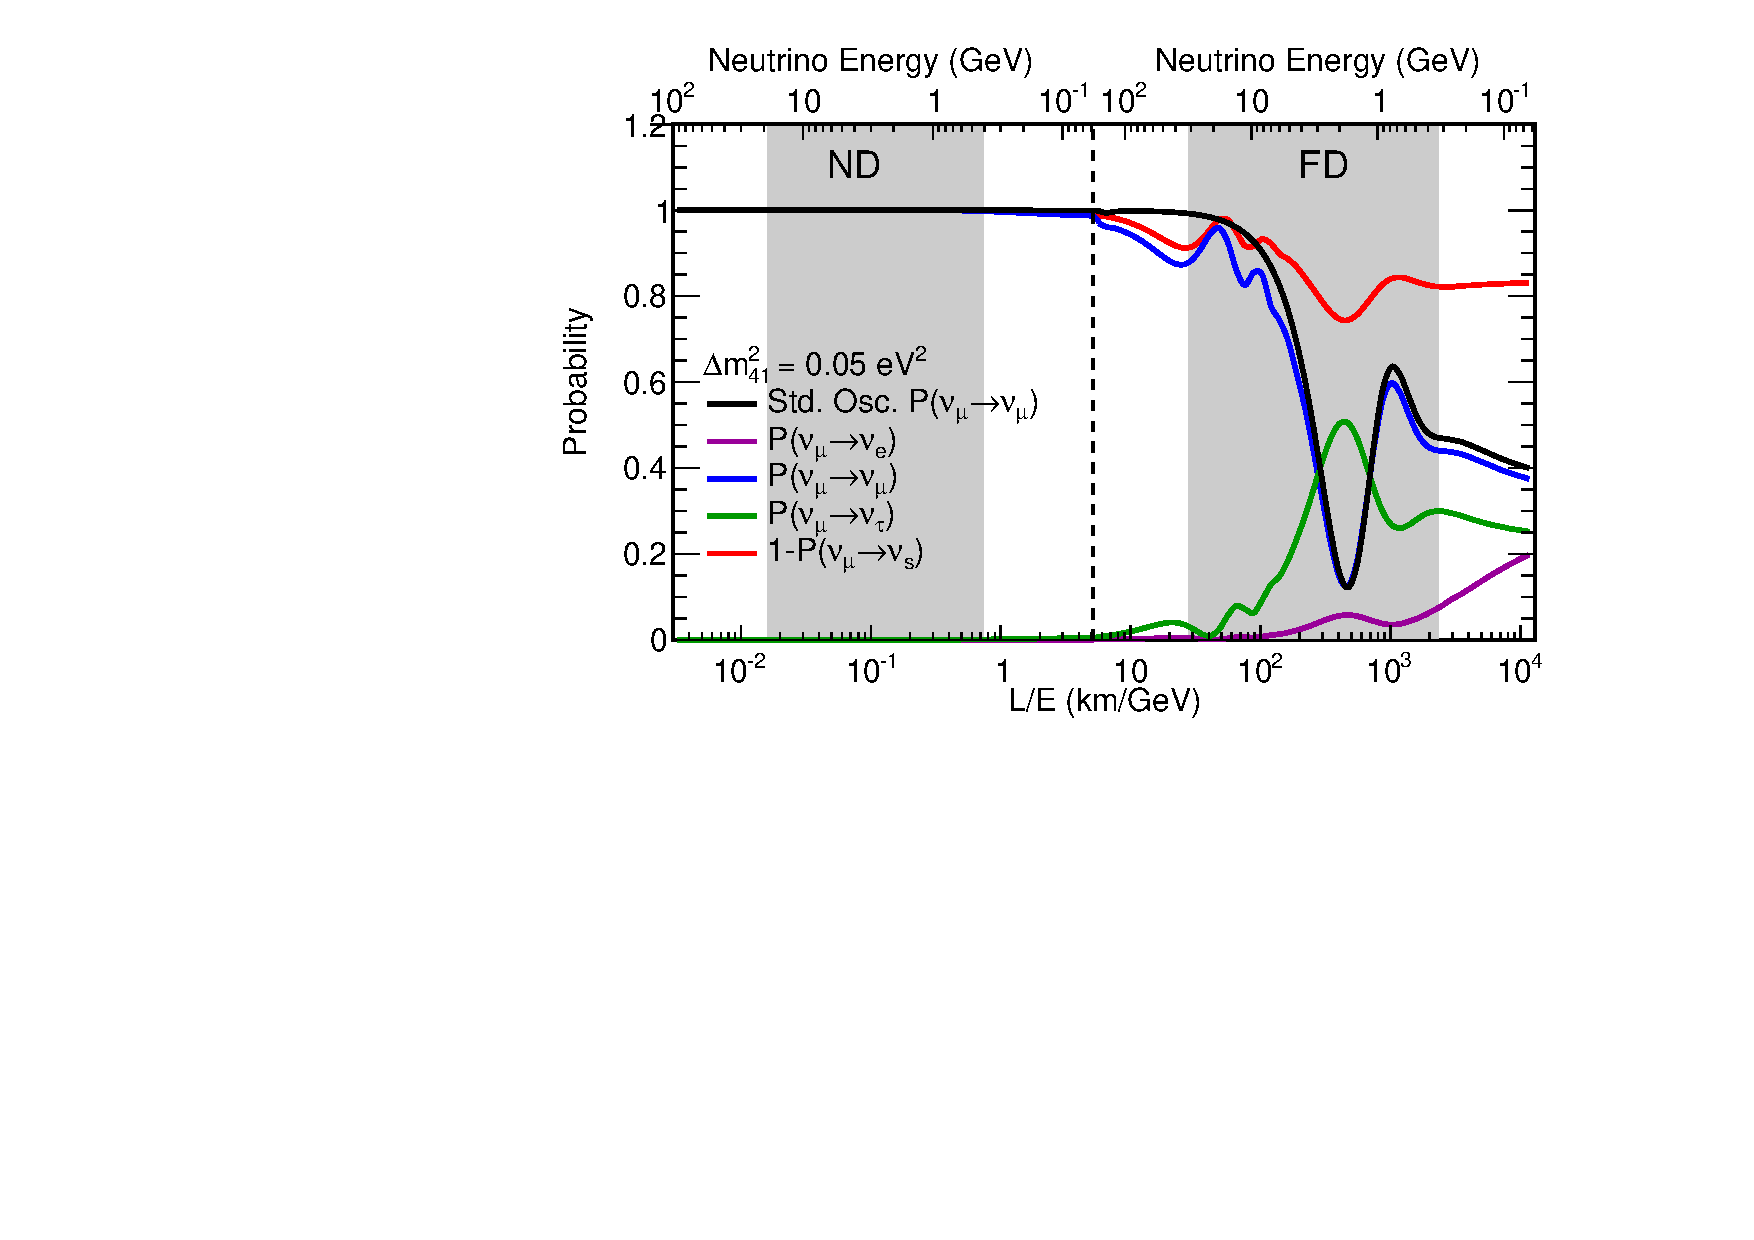
\includegraphics[width=0.49\columnwidth]{./figures/DUNE_SterileSensi_dm0_05}
%\includegraphics[width=0.49\columnwidth]{./figures/DUNE_SterileSensi_dm5}
\caption{\label{fig:LoverE} Oscillation probabilities as a function of L/E and neutrino energy for different values of $\Delta m^2_{41}$. For values of $\Delta m^2_{41} > 1\,\mathrm{eV}^2$, distortions occur at the ND baseline, spanning the L/E range probed by LSND and MiniBooNE.}
\end{figure}

Assessment of DUNE's sensitivity to mixing with light sterile neutrinos proceeds through a simultaneous ND and FD fit framework developed with GLoBES~\cite{ref:globes}.
The obtained sensitivities for the various mixing angles are shown in Figs.~\ref{fig:th_24}, \ref{fig:th_mue}, \ref{fig:th_14}, \ref{fig:th_34}. 

\begin{figure}[!htbp]
\centering
%\includegraphics[width=0.5\columnwidth]{./figures/MultiPlots_DUNE_MINOS_IceCube_globAppF_th_24}
\caption{\label{fig:th_24} DUNE 95\% C.L. limit on $\sin^2 \theta_{24}$ compared to current and previous experiments.}
\end{figure}

\begin{figure}[!htbp]
\centering
%\includegraphics[width=0.5\columnwidth]{./figures/DUNE_ComboLimit95_th_mue}
\caption{\label{fig:th_mue} DUNE 95\% C.L. limit on $\sin^2 \theta_{\mu e}$ compared to current and previous experiments.}
\end{figure}

\begin{figure}[!htbp]
\centering
%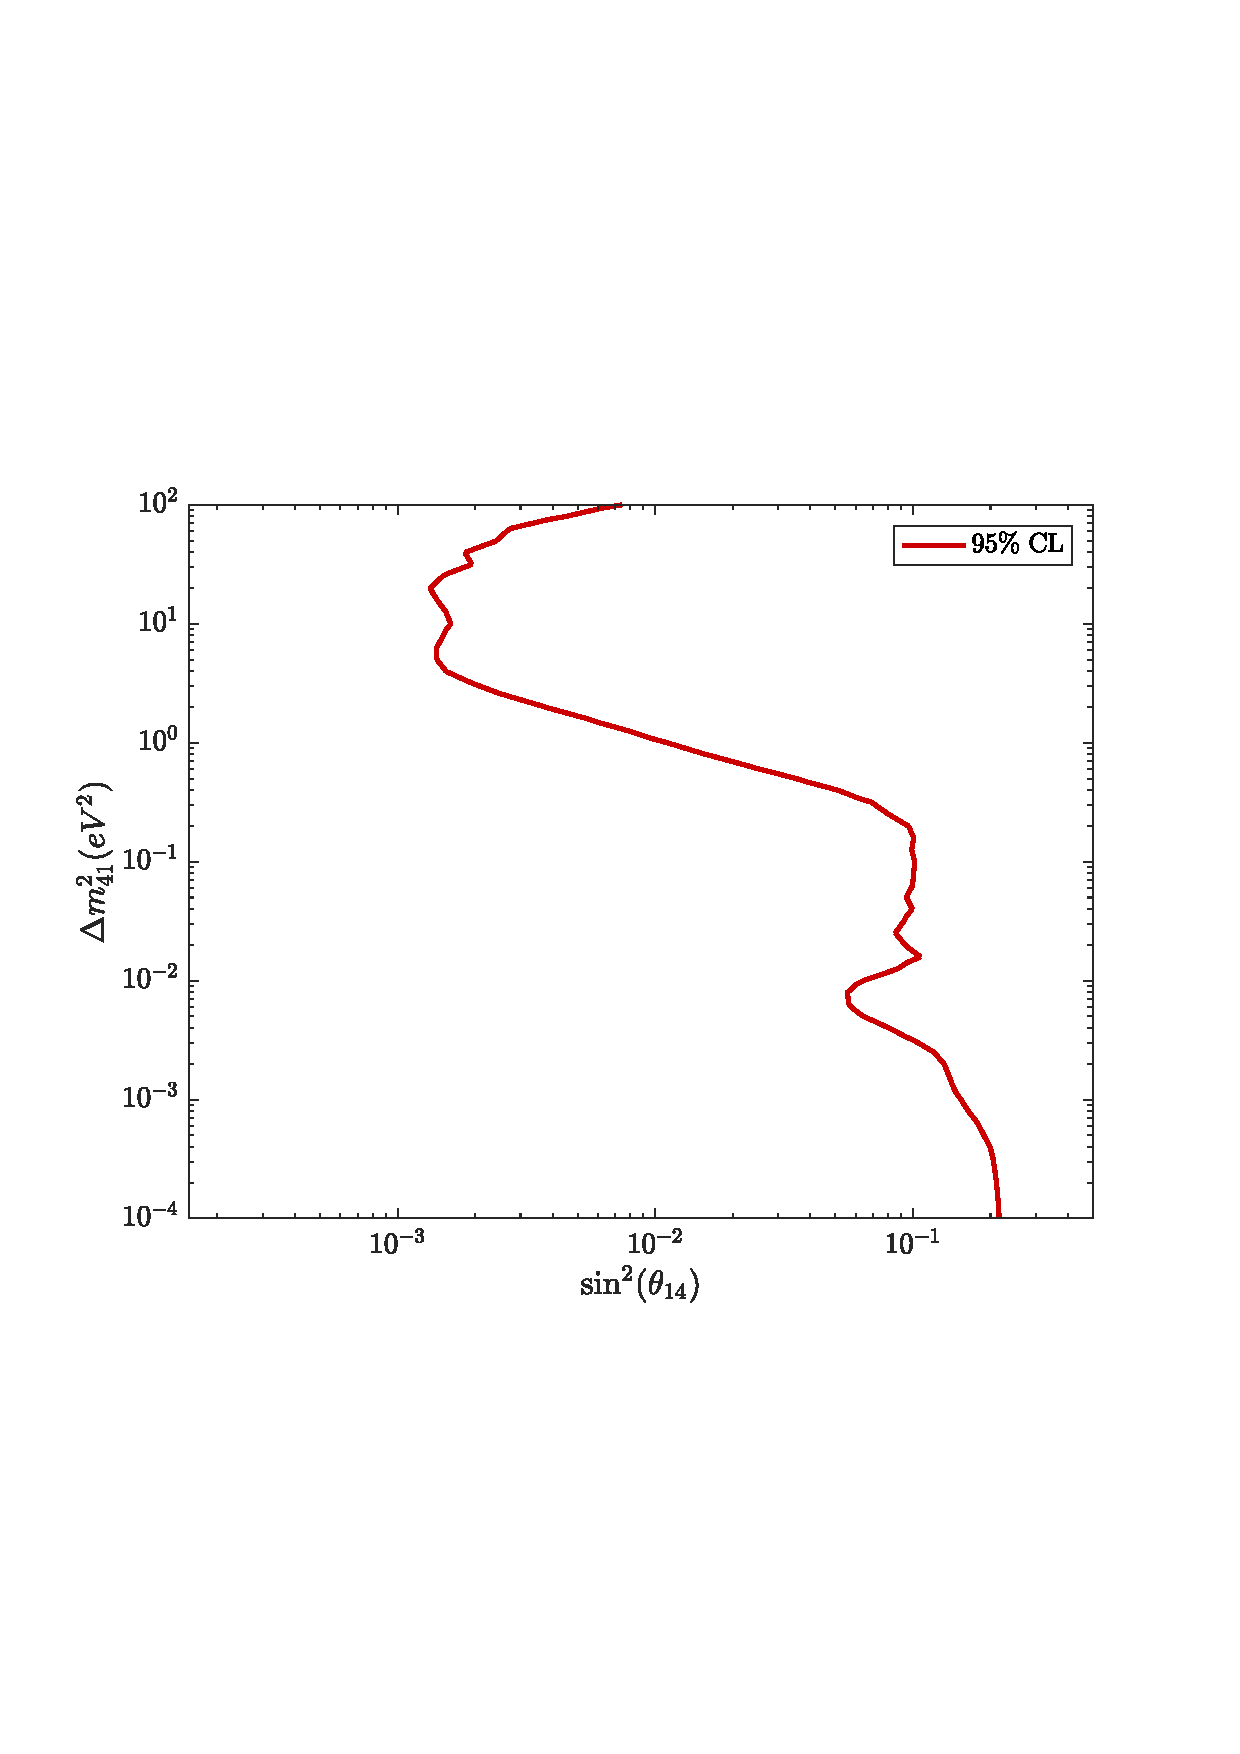
\includegraphics[width=0.4\columnwidth]{./figures/th_14}
\caption{\label{fig:th_14} DUNE 95\% C.L. limit on $\sin^2 2\theta_{14}$ compared to current and previous experiments - placeholder.}
\end{figure}

\begin{figure}[!htbp]
\centering
%\includegraphics[width=0.4\columnwidth]{./figures/th_34}
\caption{\label{fig:th_34} DUNE 95\% C.L. limit on $\sin^2 \theta_{34}$ compared to current experiments - placeholder.}
\end{figure}

\subsection{Large Extra-Dimensions}
\begin{itemize}
\item Motivation
\item Datasets, signal, background studies
\item List of Key Plots/tables
\item Results and Conclusions
\end{itemize}
DUNE can search for or constrain the size of large extra-dimensions (LED) by looking for distortions of the oscillation pattern predicted by the three-flavor paradigm. These distortions arise through mixing between the right-handed neutrino Kaluza-Klein modes, which propagate in the compactified extra dimensions, and the active neutrinos, which exist only in the four-dimensional brane~\cite{LEDModel}. Searching for these distortions in, for instance, the $\nu_\mu$~CC disappearance spectrum should provide significantly enhanced sensitivity over existing results from the MINOS/MINOS+ experiment~\cite{MinosplusLED}.


\subsection{Non-Standard Neutrino Interactions}
\begin{itemize}
\item Motivation
\item Datasets, signal, background studies
\item List of Key Plots/tables
\item Results and Conclusions
\end{itemize}

\subsection{Non-Unitary Mixing}
\begin{itemize}
\item Motivation
\item Datasets, signal, background studies
\item List of Key Plots/tables
\item Results and Conclusions
\end{itemize}

\subsection{Anomalous Long-Baseline $\nu_{\tau}$ Appearance }
\begin{itemize}
\item Motivation
\item Datasets, signal, background studies
\item List of Key Plots/tables
\item Results and Conclusions
\end{itemize}

\subsection{CPT Violation}
\begin{itemize}
\item Motivation
\item Datasets, signal, background studies
\item List of Key Plots/tables
\item Results and Conclusions
\end{itemize}






%%%%%%%%%%%%%%%%%%%%%%%%%%%%%%%%%%%%%%%%%%%%%%%%%%%%%%%%%%%%%%
\section{Non-accelerator physics capitalizing on DUNE far detector capabilities}\label{sec:bsm-nonaccel}
\begin{itemize}
\item General Motivation
\item Software Tools
\end{itemize}

\subsection{Boosted Dark Matter}
\begin{itemize}
\item Motivation
\item Datasets, signal, background studies
\item List of Key Plots/tables
\item Results and Conclusions
\end{itemize}

%%%%%%%%%%%%%%%%%%%%%%%%%%%%%%%%%%%%%%%%%%%%%%%%%%%%%%%%%%%%%%
\section{BSM physics opportunities with the near detector}\label{sec:bsm-nd}
\begin{itemize}
\item General Motivation
\item Near detector assumptions
\item Software Tools
\end{itemize}

\subsection{Low-Mass Dark Matter}
\begin{itemize}
\item Motivation
\item Datasets, signal, background studies
\item List of Key Plots/tables
\item Results and Conclusions
\end{itemize}

\subsection{Heavy Neutral Leptons}
\begin{itemize}
\item Motivation
\item Datasets, signal, background studies
\item List of Key Plots/tables
\item Results and Conclusions
\end{itemize}

\subsection{Neutrino Tridents}
\begin{itemize}
\item Motivation
\item Datasets, signal, background studies
\item List of Key Plots/tables
\item Results and Conclusions
\end{itemize}
The intriguing possibility that neutrinos may be charged under new gauge symmetries beyond the Standard Model (SM) $SU(3)_c\times SU(2)_L\times U(1)_Y$, and interact with the corresponding new gauge bosons can be tested with unprecedented precision by DUNE through near detector measurements of neutrino-induced di-lepton production in the Coulomb field of a heavy nucleus, also known as {\it neutrino trident} interactions~\cite{Altmannshofer:2014pba}. Although this process is extremely rare (SM rates are suppressed by a factor of $\sim 10^{-5}-10^{-7}$ with respect to CC interactions), the CHARM-II collaboration \cite{Geiregat:1990gz} and the CCFR collaboration \cite{Mishra:1991bv} both reported detection of several trident events ($\sim 40$ events at CCFR) and quoted cross-sections in good agreement with the SM predictions. With a predicted annual rate of over 100 di-muon neutrino trident interactions at the near detector, DUNE will be able to measure deviations from the SM rates and test for the presence of new gauge symmetries.

\subsection{Short-Baseline Sterile Neutrino Mixing}
\begin{itemize}
\item Motivation
\item Datasets, signal, background studies
\item List of Key Plots/tables
\item Results and Conclusions
\end{itemize}